%CLASSE DOCUMENTO - LINGUA E DIMENSIONE FONT
\documentclass[12pt, cucitura]{toptesi}

%%%%%%%%%%%%%%%%%%%%%%%%%%%%%%%%%%%%%%%%%%%%%%%%%%%%%%%%%%%%%%%

% INCLUSIONE PACCHETTI
\usepackage[utf8]{inputenc} %utf8
\usepackage[italian]{babel}
\usepackage[T1]{fontenc}
\usepackage{blindtext}
\usepackage{graphicx,wrapfig}
\usepackage{booktabs}
\usepackage{lmodern}
\usepackage{varioref}
\usepackage{url}
\usepackage{array}
\usepackage{paralist}{\obeyspaces\global\let =\space}
\usepackage{verbatim} 
\usepackage{subfig}
\usepackage{tabularx}
\usepackage{amsmath}
\usepackage{amsfonts}
\usepackage{float}
\usepackage{amssymb}
\usepackage{multicol}
\usepackage{multirow}
\usepackage{listings}
\usepackage[pass]{geometry}
\usepackage[figuresright]{rotating}
\usepackage{algorithm}
\usepackage{algorithmic}
\usepackage{amsmath}
\usepackage[babel]{csquotes}
\usepackage{hyperref}
\usepackage[backend=bibtex]{biblatex}
\usepackage{color}
\usepackage{xcolor}
\usepackage{adjustbox}

\definecolor{lightgray}{rgb}{.9,.9,.9}
\definecolor{darkgray}{rgb}{.4,.4,.4}
\definecolor{purple}{rgb}{0.65, 0.12, 0.82}
\colorlet{punct}{red!60!black}
\definecolor{background}{HTML}{F1F3F4}
\definecolor{delim}{RGB}{20,105,176}
\colorlet{numb}{magenta!60!black}

%%%%%%%%%%%%%%%%%%%%%%%%%%%%%%%%%%%%%%%%%%%%%%%%%%%%%%%%%%%%%%%

% CONFIGURAZIONE LINK E RIFERIMENTI
\hypersetup{%
    pdfpagemode={UseOutlines},
    bookmarksopen,
    pdfstartview={FitH},
    colorlinks,
    linkcolor={black}, %COLORE DEI RIFERIMENTI AL TESTO
    citecolor={blue}, %COLORE DEI RIFERIMENTI ALLE CITAZIONI
    urlcolor={black} %COLORI DEGLI URL
}

%%%%%%%%%%%%%%%%%%%%%%%%%%%%%%%%%%%%%%%%%%%%%%%%%%%%%%%%%%%%%%%

% CONFIGURAZIONE LISTATI/CODICE - CANCELLARE SE NON NECESSARIO

\lstdefinelanguage{JavaScript}{
  keywords={typeof, new, true, false, catch, function, return, null, catch, switch, var, let, const, if, in, while, do, else, case, default, break},
  keywordstyle=\color{blue}\bfseries,
  ndkeywords={class, export, boolean, throw, implements, import, this},
  ndkeywordstyle=\color{darkgray}\bfseries,
  identifierstyle=\color{black},
  sensitive=false,
  comment=[l]{//},
  morecomment=[s]{/*}{*/},
  commentstyle=\color{purple}\ttfamily,
  stringstyle=\color{red}\ttfamily,
  morestring=[b]',
  morestring=[b]"
}

\lstdefinelanguage{json}{
    basicstyle=\normalfont\ttfamily,
    numbers=left,
    numberstyle=\scriptsize,
    stepnumber=1,
    numbersep=8pt,
    showstringspaces=false,
    breaklines=true,
    frame=none,
    literate=
     *{0}{{{\color{numb}0}}}{1}
      {1}{{{\color{numb}1}}}{1}
      {2}{{{\color{numb}2}}}{1}
      {3}{{{\color{numb}3}}}{1}
      {4}{{{\color{numb}4}}}{1}
      {5}{{{\color{numb}5}}}{1}
      {6}{{{\color{numb}6}}}{1}
      {7}{{{\color{numb}7}}}{1}
      {8}{{{\color{numb}8}}}{1}
      {9}{{{\color{numb}9}}}{1}
      {:}{{{\color{punct}{:}}}}{1}
      {,}{{{\color{punct}{,}}}}{1}
      {\{}{{{\color{delim}{\{}}}}{1}
      {\}}{{{\color{delim}{\}}}}}{1}
      {[}{{{\color{delim}{[}}}}{1}
      {]}{{{\color{delim}{]}}}}{1},
}

\lstdefinestyle{JavaScriptStyle}{
    captionpos=b,
	language=JavaScript,
	basicstyle =\small\ttfamily,
	breaklines=true,
	breakatwhitespace=true,
	frame=none,
	numbers=left,
	numberstyle=\footnotesize,
	aboveskip=20pt,
	belowskip=10pt,
	lineskip=3pt,
	showstringspaces=false,
}

\lstdefinestyle{JsonStyle}{
    captionpos=b,
	language=json,
	basicstyle =\small\ttfamily,
	breaklines=true,
	breakatwhitespace=true,
	frame=none,
	numbers=left,
	numberstyle=\footnotesize,
	aboveskip=20pt,
	belowskip=10pt,
	lineskip=4pt,
	showstringspaces=false
}

%%%%%%%%%%%%%%%%%%%%%%%%%%%%%%%%%%%%%%%%%%%%%%%%%%%%%%%%%%%%%%%

% FRENCHSPACING VA _SEMPRE_ ABILITATO PER DOCUMENTI IN ITALIANO
\frenchspacing

%%%%%%%%%%%%%%%%%%%%%%%%%%%%%%%%%%%%%%%%%%%%%%%%%%%%%%%%%%%%%%%

%DEFINIZIONE SEZIONI IN NUMERAZIONE ROMANA
%ELENCO DEI LISTATI/CODICI
\makeatletter
\newcommand\listofcodes{%
 \iffrontmatter\else\frontmattertrue\fi
 \if@openright\cleardoublepage\else\clearpage\fi
 % change the meaning of \chapter in a group
 \begingroup\def\chapter##1{\@schapter}
 \phantomsection % for the hyperlink
 \lstlistoflistings 
 \endgroup
} 
\makeatother

%%%%%%%%%%%%%%%%%%%%%%%%%%%%%%%%%%%%%%%%%%%%%%%%%%%%%%%%%%%%%%%

% INFORMAZIONI PDF - PERSONALIZZARE
\pdfinfo{%
  /Title    (OVL DASHBOARD)
  /Author   (Lorenzo Diato)
  /Keywords (Tesi di Laurea in Informatica Themis)
}

%%%%%%%%%%%%%%%%%%%%%%%%%%%%%%%%%%%%%%%%%%%%%%%%%%%%%%%%%%%%%%%

% FRONTESPIZIO - PERSONALIZZARE
% ELIMINATE LE VOCI CHE NON VI SERVONO

% UNIVERSITA - NOME
\ateneo{\Large{\textbf{Universita degli Studi di Torino}}}

% FACOLTA - DICITURA - CANCELLARE O DECOMMENTARE
\FacoltaDi{\Large{\textbf{Dipartimento di }}}
% FACOLTA - NOME
\facolta{\Large{\textbf{Informatica}}}

% CORSO DI LAUREA - NOME
\corsodilaurea{Informatica}

% LOGO UNIVERSITA
\logosede[50mm]{images/logo}

%binding correction
\setbindingcorrection{7mm}

% TIPOLOGIA TESI
\TesiDiLaurea{\Large{Tesi di Laurea Triennale in Informatica}}

% TITOLO
\titolo{SVILUPPO OVL DASHBOARD}
				
% RELATORE/I - DICITURA - CANCELLARE SE UN SOLO RELATORE
% RELATORE - PROF. NOME E COGNOME
\relatore{Prof.ssa\ Giovanna Petrone}

% TUTORE AZIENDALE - TITOLO NOME E COGNOME
\tutoreaziendale{Dott. Bruno Cavigioli}
% TUTORE AZIENDALE - DICITURA//AZIENDA
\NomeTutoreAziendale{Tutor Aziendale\\Themis s.r.l}

% CANDIDATO - DICITURA (MANTENERE I DUE PUNTI) - CANCELLARE O DECOMMENTARE
%\CandidateName{Candidate:}

% CANDIDATO - NOME E COGNOME
\candidato{Lorenzo Diato}

% DATA - MESE ANNO
\sedutadilaurea{ANNO ACCADEMICO 2018-19}

%%%%%%%%%%%%%%%%%%%%%%%%%%%%%%%%%%%%%%%%%%%%%%%%%%%%%%%%%%%%%%%

% LISTA DEI CAPITOLI DA INCLUDERE - PERSONALIZZARE
\includeonly{%
introduzione,%
descrizione_del_progetto,
frontend,
backend,
conclusioni
}

% FILE DI BIBLIOGRAFIA
\bibliography{bibliography} 

%%%%%%%%%%%%%%%%%%%%%%%%%%%%%%%%%%%%%%%%%%%%%%%%%%%%%%%%%%%%%%%

% INIZIO DOCUMENTO
\begin{document}

\frontespizio

%%%%%%%%%%%%%%%%%%%%%%%%%%%%%%%%%%%%%%%%%%%%%%%%%%%%%%%%%%%%%%%

%INTERLINEA - DEFAULT 1 - NON ESAGERATE, NON SUPERATE MAI 1.3 ;)
\interlinea{1.2}

%%%%%%%%%%%%%%%%%%%%%%%%%%%%%%%%%%%%%%%%%%%%%%%%%%%%%%%%%%%%%%%

% RINGRAZIAMENTI - PERSONALIZZARE
\ringraziamenti
Ringrazio la mia relatrice, la professoressa Giovanna Petrone, per la
cordialità e la professionalità con cui mi ha seguito durante la
realizzazione di questo lavoro. Ringrazio inoltre il Dott. Bruno Cavigioli per
avermi aiutato anch’egli nella creazione del sito e nella stesura dell’elaborato.
Vorrei ingraziare la mia famiglia che mi ha sempre sostenuto durante il percorso di studi e mi ha permesso di raggiungere questo risultato. Per ultimi, ma non meno importanti, il mio gruppo di amici con i quali ho frequentato e studiato e grazie al quale ho sempre trovato motivazione e ottimi consigli.

%%%%%%%%%%%%%%%%%%%%%%%%%%%%%%%%%%%%%%%%%%%%%%%%%%%%%%%%%%%%%%%

% INDICI - ELIMINARE GLI INDICI NON NECESSARI

% INDICE GENERALE
\tableofcontents

% INDICE DELLE FIGURE
%\listoffigures

% INDICE DELLE TABELLE
%\listoftables

% INDICE DEI CODICI
%\listofcodes

%%%%%%%%%%%%%%%%%%%%%%%%%%%%%%%%%%%%%%%%%%%%%%%%%%%%%%%%%%%%%%%

\mainmatter

% INCLUSIONE FILE CAPITOLI - PERSONALIZZARE - TENERE COERENTE CON LISTA IN ALTO
\chapter{introduzione}
\label{chap:introduzione}

\section{Ambito del progetto}
\label{sec:ambito del progetto}

Il presente lavoro ha come oggetto lo studio dello sviluppo e della progettazione della piattaforma OVL Dashboard, un portale che permette la gestione e il monitoraggio di una rete virtuale di dispositivi situati in diverse strutture sanitarie su tutto il territorio italiano. Questo progetto è stato realizzato all’interno dell’azienda Themis, durante il mio stage curricolare, ed ha richiesto circa tre mesi per la sua realizzazione.
Il sito è accessibile da chiunque possegga un account registrato alla piattaforma, la cui creazione avviene tramite invito. Un utente registrato può essere in grado di accedere alle macchine collegate alla rete OVL, modificarne le proprietà o interagire con altri utenti in base ai permessi da esso posseduti.
Ho scelto dall’elenco delle proposte di stage disponibili proprio questa in quanto sono sempre interessato alle tecnologie che permettono la migrazione in cloud di servizi di uso quotidiano. Inoltre, questo stage mi offriva la possibilità di applicare concretamente le mie competenze di full-stack developer e svilupparle in un contesto lavorativo.
Per la realizzazione di tale progetto ho utilizzato diverse tecnologie tra le quali JavaScript in particolare la libreria ReactJS, NodeJS, MySQL, MongoDB, Git.

\section{Descrizione dell'azienda}
\label{sec:descrizione dell'azienda}

La società Themis s.r.l. nasce nell’incubatore del Politecnico di Torino nell’anno 2004, come evoluzione da realtà professionali e da altre società che hanno come filo conduttore l’attività d’ingegneria del software, nata come UNO s.r.l. nel 1981. Dalla sua nascita, Themis interviene nell’organizzazione e management di progetti per l’automazione di sistemi complessi su specifiche che non hanno riscontro in soluzioni pronte nel settore I.T. e nella  raccolta, distribuzione e gestione di dati e condivisione delle risorse, integrando i propri prodotti con le tecnologie più innovative che utilizzano il cloud come naturale centro nodale delle proprie piattaforme.
\chapter{Descrizione del progetto}
\label{chap:descrizione del progetto}

\section{Requisiti della piattaforma}
\label{sec:requisiti della piattaforma}

La piattaforma è stata ideata con una serie di funzionalità e caratteristiche che le consentono di raggiungere i propri obiettivi, cercando di essere al contempo semplice da utilizzare per l’utente finale.

\subsection{Utenti}
\label{sec:utenti}

Sono stati pensati tre livelli di utenti ognuno con accesso a risorse e permessi differenti:
\begin{itemize}
    \item super-utente (utente aziendale Themis) è l'utente unico: ha accesso a tutte le risorse.  Esso può visualizzare, modificare ed eliminare le connessioni, gli utenti e i relativi permessi che essi hanno in modo da abilitare o precludere l'accesso a determinate connessioni
    \item amministratore: ha accesso ad un sottogruppo di connessioni e può proporre la modifica di una connessione che può visualizzare
    \item utente base: può visualizzare e accedere ad un sottogruppo di connessioni
\end{itemize}

Ogni utente è caratterizzato, inoltre, da un ruolo che rispecchia l'incarico professionale che esso possiede (amministratore, tecnico, medico, medico specialista). Questo attributo trova la sua funzione nel momento in cui un certo utente ha necessità di una consulenza mediante la pagina di consulenza real-time. In genere, il livello amministratore è assegnato ovviamente al singolo ruolo amministratore, mentre i rimanenti ruoli sono utenti base.

\subsection{Connessioni e gruppi}
\label{sec:connessioni e gruppi}

Per gestire le connessioni è stata rispettata la struttura ad albero che lega gerarchicamente i dispositivi appartenenti alla rete di Guacamole. Le connessioni possono appartenere ad un gruppo e, i gruppi sono organizzati tra loro in modo da rispecchiare il più fedelmente possibile la locazione geografica e le strutture in cui sono presenti i dispositivi collegati alla rete. Grazie a questa struttura, è possibile assegnare agli utenti interi gruppi oppure poche particolari connessioni determinando così i dispositivi a cui può accedere.
La relazione esistente tra gli utenti e i loro permessi, su connessioni e gruppi, dona ad essi un'implicita struttura gerarchica che ha come radice l'account super-utente, procedendo man mano con amministratori e tutti gli utenti base. Si può pensare agli account amministratori ognuno come gestore di un particolare ramo di connessioni, cioè di un determinato gruppo. Un gruppo rappresenta una struttura sanitaria, ben localizzata, al cui interno sono stati configurati dispositivi interfacciati alla rete virtuale OVL. 

\begin{figure}
\begin{center}
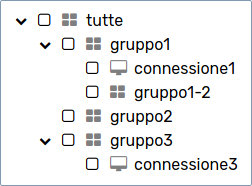
\includegraphics{main/images/tree.png}
\end{center}
\caption{Struttura delle connessioni.}
\label{fig:tree}
\end{figure}

La figura precedente rappresenta un esempio di albero di connessioni.
Sotto la radice \textit{tutte} è possibile notare tre differenti nodi che rappresentano gruppi di connessioni. In genere, i gruppi dell'albero aventi livello di profondità uno delineano ognuno regioni geografiche, mentre quelli di livello due rappresentano le strutture mediche. La maggior parte delle connessioni, quindi, fanno riferimento a struttura e regione ben definite. 

\subsection{Casi d'uso}
\label{sec:casi d'uso}

\begin{center}
\begin{tabular}{c c c c}
\textbf{Operazioni} & \textbf{Super-utente} & \textbf{Amministratore} & \textbf{Utente}\\
\midrule
\textbf{Connessioni}\\
Visualizzazione connessioni & SI & SI & SI\\
Accesso remoto connessioni & SI & SI & SI\\
Aggiunta connessione & SI & Su richiesta & NO\\
Modifica connessione & SI & Su richiesta & NO\\
Eliminazione connessione & SI & Su richiesta & NO\\
\midrule
\textbf{Gruppi}\\
Visualizzazione gruppi & SI & SI & SI\\
Aggiunta gruppo & SI & NO & NO\\
Modifica gruppo & SI & NO & NO\\
Eliminazione gruppo & SI & NO & NO\\
\midrule
Invito utenti & SI & SI & SI\\
Ricerca database & SI & NO & NO\\
Modifica permessi utenti & SI & NO & NO\\
Richiesta comunicazione  & SI & SI & SI
\end{tabular}
\end{center}

Nella tabella sono riportate le operazioni che ciascun livello di utente può eseguire. Alcune di queste sono già state trattate nei paragrafi precedenti, ma in questo caso la tabella risulta utile per avere un quadro completo dei permessi che ciascun utente possiede.
Nel caso delle voci di visualizzazione di connessioni, dei gruppi e di accesso remoto alle connessioni, il valore riferito all'utente base dipende dalle connessioni che gli sono state assegnate al momento dell'invito. Se non viene selezionata alcuna connessione dall'albero, l'utente non potrà accedere e visualizzare alcuna connessione.

\section{Aspetto della piattaforma}
\label{sec:aspetto della piattaforma}

\subsection{Invito utenti}
\label{sec:invito utenti}
Per partecipare alla piattaforma e per poter accedere ai suoi contenuti è necessario effettuare l’iscrizione, che può essere intrapresa solo tramite invito effettuato da un utente già registrato.
La pagina visualizzata al momento dell'apertura della dashboard, dopo aver effettuato il login, è dedicata appunto all'operazione di invito di nuovi utenti. 

\begin{figure}
\begin{center}
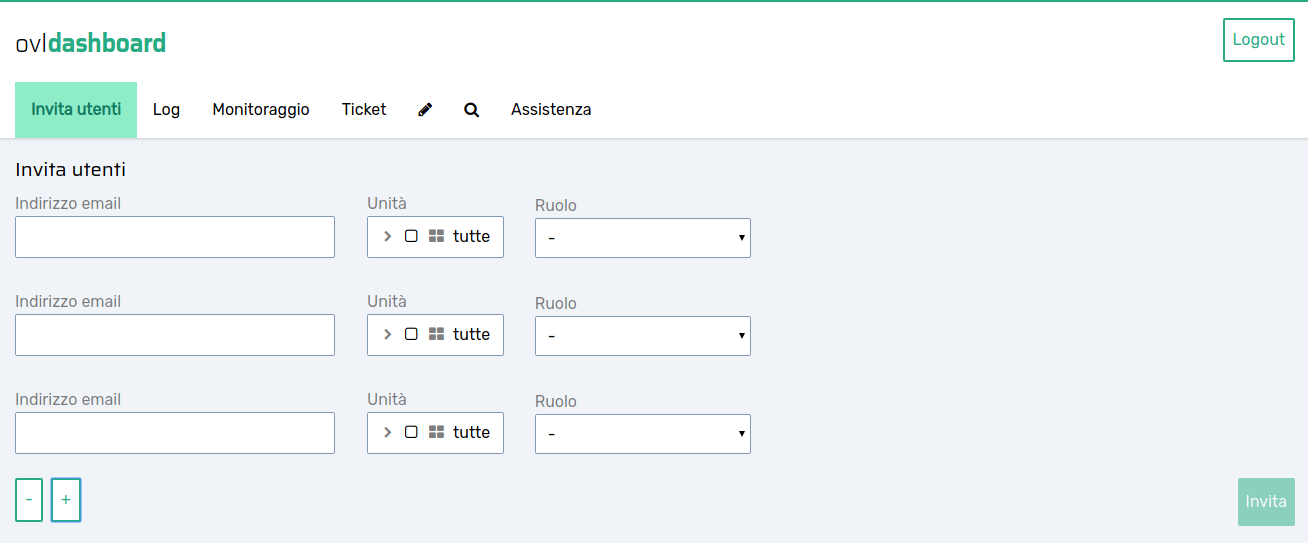
\includegraphics[scale=0.43]{main/images/invitations.png}
\end{center}
\caption{Pagina di invito nuovi utenti.}
\label{fig:invitations}
\end{figure}

La pagina mostra una prima area di input in cui è possibile inserire l'indirizzo e-mail della persona che si desidera invitare ad utilizzare la piattaforma. Successivamente, si indicano le connessioni ed i gruppi a cui il nuovo utente potrà accedere (utilizzando la struttura ad albero precedentemente illustrata) e il ruolo che esso ricopre.
Il numero delle richieste di invito che si desidera effettuare può essere incrementato aggiungendo nuovi form mediante l'apposito tasto.
Procedendo con la conferma verrà inviata una mail (con richiesta al server di autorizzazione) a tutti gli indirizzi precedentemente indicati, ed i rispettivi utenti provvederanno al completamento della registrazione.

Se un invito viene effettuato esplicitando \textit{amministratore} come valore del campo ruolo, il nuovo utente verrà registrato sulla piattaforma con permessi di modifica e eliminazione sulle sole connessioni a cui egli ha accesso.

\subsection{Form connessioni e gruppi}
\label{sec:form connessioni e gruppi}
L'aggiunta di una nuova connessione viene effettuata attraverso un form nel quale l'utente deve specificare caratteristiche e parametri del dispositivo da aggiungere. Tali dati servono al sistema di Guacamole per instaurare la connessione con successo. In particolare, occorre specificare il gruppo a cui la nuova connessione dovrebbe appartenere. 

\begin{figure}
\begin{center}
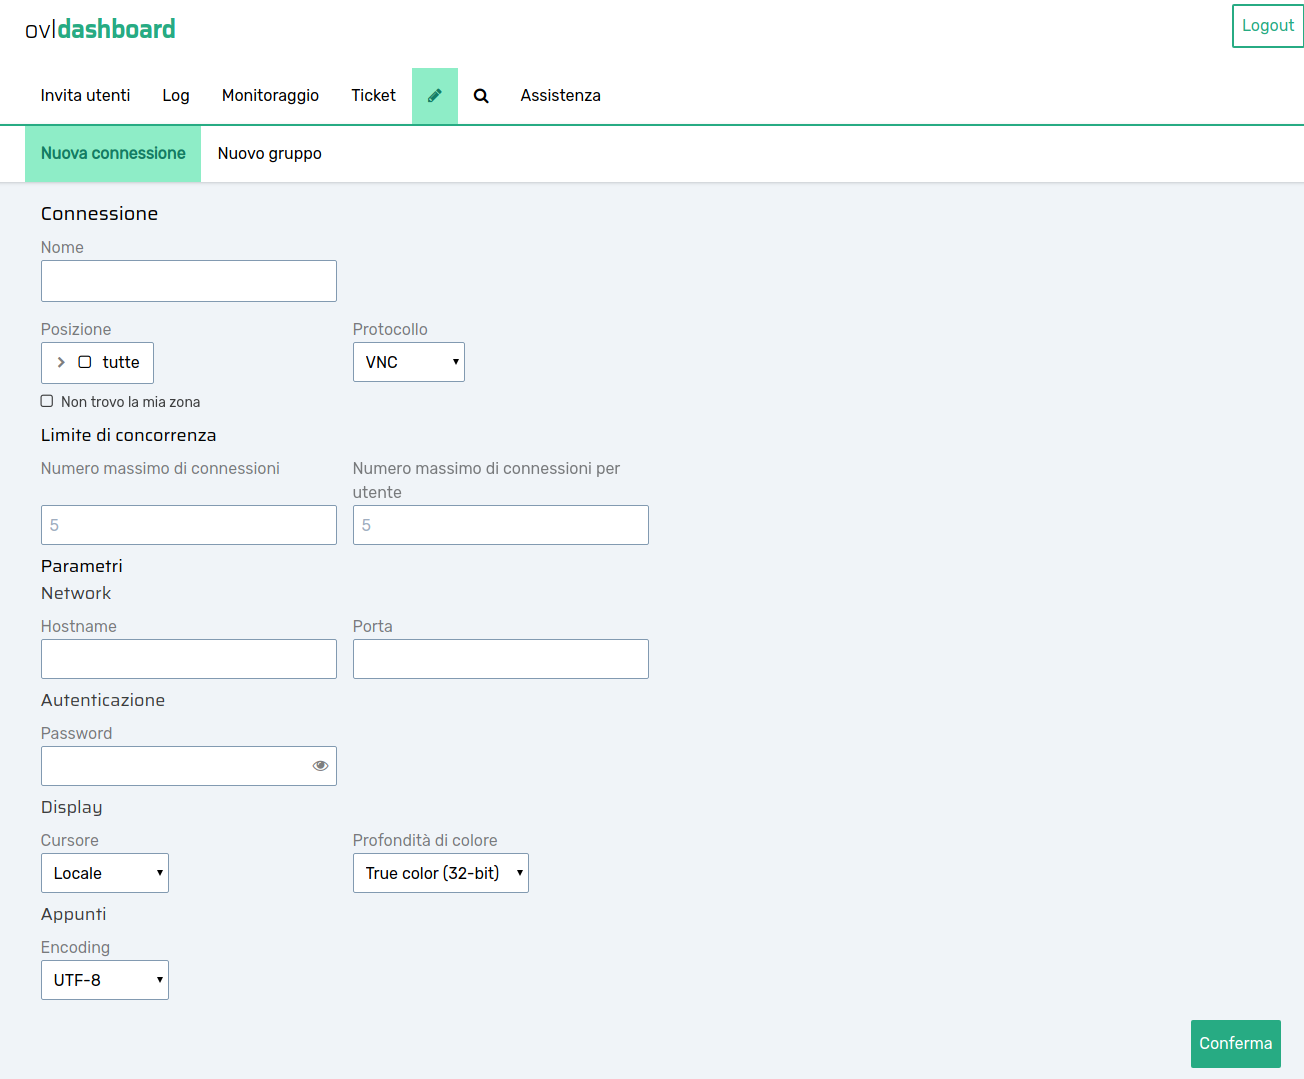
\includegraphics[scale=0.40]{main/images/form.png}
\end{center}
\caption{Form di aggiunta nuova connessione.}
\label{fig:connectionForm}
\end{figure}

L'intera pagina è visibile da tutti gli utenti aventi ruolo amministratore, ma l'inserimento diretto di una nuova connessione nel sistema viene permesso soltanto al super-utente aziendale Themis. 

Al momento della pressione del pulsante di conferma da parte di un utente amministratore, i parametri digitati vengono raccolti ed organizzati sottoforma di richiesta nella pagina \textit{ticket} (questo concetto viene spiegato meglio nella sezione successiva) che verrà approvato o rifiutato in un secondo momento. Se, invece, l'account con cui è stato effettuato il login è quello super-utente, l'azione di conferma crea la nuova connessione fin da subito e sarà disponibile nell'albero e in tutto il sistema.
La differenziazione tra account super-utente e account amministratore è stata mantenuta in ogni caso d'uso riguardante le connessioni: il ticket di richiesta viene creato ogni volta che un utente amministratore ha l'esigenza di aggiungere, modificare o eliminare una connessione sistema. 

Un altro privilegio che possiede l'account super-utente è il fatto di poter visualizzare un altro form dedicato alla gestione dei gruppi avente funzionalità di aggiunta, modifica ed eliminazione parallele a quelle delle connessioni.

Nel caso particolare in cui un utente amministratore deve inserire una connessione per un dispositivo, situato in una località ancora non gestita come gruppo all'interno della piattaforma, può specificare all'interno del form un recapito. Questa informazione permette all'account super-utente di contattare, al momento della gestione del ticket, l'autore della richiesta e, quindi, di aggiungere il gruppo necessario all'inserimento della connessione.

\subsection{Ticket}
\label{sec:ticket}
La pagina dei ticket è strettamente legata alla creazione di nuove connessioni. Questa, infatti, raccoglie tutte le richieste generate dagli utenti amministratori. 
Le richieste vengono generate ogni volta che un utente amministratore desidera aggiungere, modificare o eliminare una connessione. Ogni richiesta viene presentata sottoforma di ticket.

\begin{figure}
\begin{center}
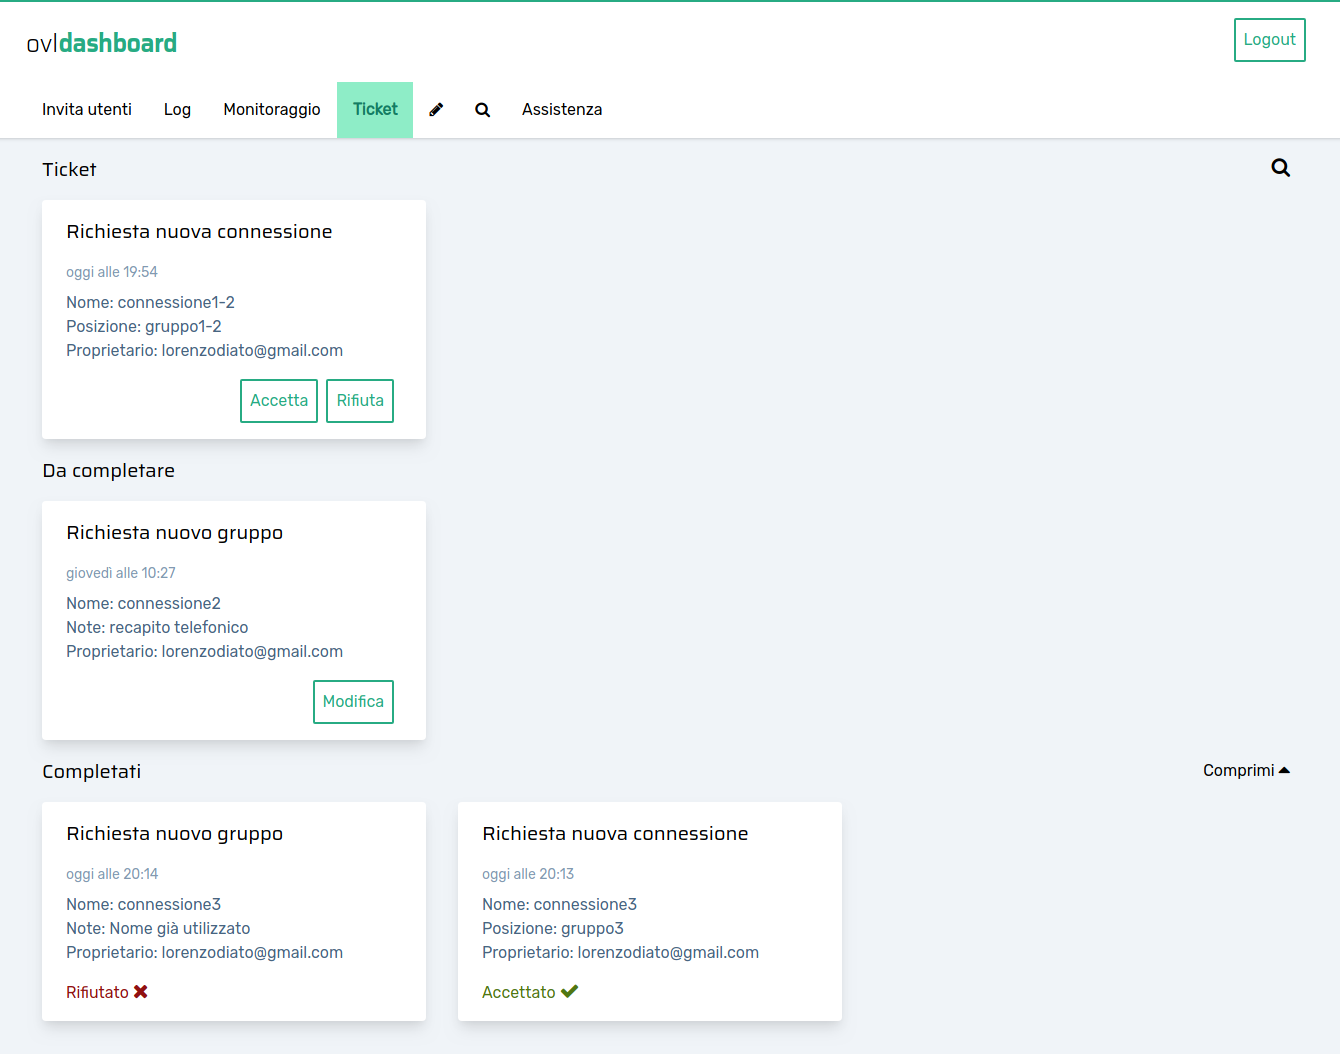
\includegraphics[scale=0.40]{main/images/tickets.png}
\end{center}
\caption{Pagina dei ticket.}
\label{fig:tickets}
\end{figure}

La pagina è suddivisa in tre sezioni: la prima, in alto, mostra i ticket ancora in attesa di riscontro (da accettare o da rifiutare); la seconda, con la dicitura \textit{da completare}, presenta quelli elaborati e presi in carico, ma in attesa di completamento. Infine, l'ultima, in basso, contiene quelli completati e consente di tenere uno storico delle richieste.
Nell'immagine sono presenti due principali tipologie di ticket: le richieste per connessioni di cui si conosce la posizione quindi il gruppo a cui dovrebbe appartenere e le richieste di connessioni il cui gruppo non esiste ancora nell'albero. Nel primo caso, gli utenti che possono risolvere la richiesta, quindi accettarla o rifiutarla sono gli amministratori più importanti dal punto di vista gerarchico e l'account super-utente. Il secondo caso, invece più complesso, può essere gestito solamente dal super-utente che provvede ad aggiungere il gruppo necessario e di conseguenza assegnarlo alla nuova connessione espressa nella richiesta.

In caso di rifiuto della richiesta l'utente deve specificare la motivazione per cui è stata effettuata quella scelta ed eventualmente come risolvere il problema. Le connessioni corrispondenti ai ticket accettati, invece, vengono inserite nel sistema e quindi subito disponibili per il collegamento remoto.

All'interno della pagina è stata implementato un filtro di ricerca: i ticket possono essere organizzati per tipologia, stato corrente o ricercati semplicemente secondo il loro nome.

\subsection{Comunicazione e assistenza}
\label{sec:comunicazione e assistenza}

La porzione di progetto descritta in questo paragrafo è stata progettata da entrambi i componenti del team di sviluppo. Io, in particolare, mi sono occupato del back-end e della creazione di una "demo" funzionante che ha velocizzato l'effettiva implementazione all'interno della dashboard. 

La pagina di assistenza offre all'utente la possibilità di contattare altri utenti mediante chat oppure chiamata vocale. In primo piano viene mostrato l'elenco degli utenti che è possibile contattare suddivisi tra account aventi una sessione attiva e account offline.
Nel caso in cui l'utente che si desidera contattare non fosse online, gli viene inviata un'email che notifica l'avvenuto tentativo di comunicazione e che contiene il collegamento d'accesso alla piattaforma. Quando viene eseguito l'accesso, l'utente viene reindirizzato direttamente alla pagina di assistenza con la comunicazione già inizializzata.
\chapter{Tecnologie di sviluppo del front-end}
\label{chap:tecnologie di sviluppo del frontend}

Per rendere lo sviluppo della dashboard più rapido e fluido si è deciso di adottare un framework web. La scelta è ricaduta sulla libreria ReactJS e sull'ottima integrazione con Redux che ha permesso più semplice l'organizzazione e il riutilizzo del codice.

\section{React}
\label{sec:react}

React è una libreria JavaScript per lo sviluppo di interfacce sviluppata da Facebook Inc. e rilasciata pubblicamente nel giugno 2013.
Secondo la definizione ufficiale data dai suoi stessi sviluppatori, React è una singola libreria interamente focalizzata alla realizzazione di interfacce grafiche. La forza di React rispetto ad altre librerie è quella di consentire l’uso di un approccio dichiarativo simile alla sintassi HTML, quindi molto familiare, per definire i componenti che rappresentano parti significative e logiche dell’interfaccia utente, ad esempio un commento a un articolo, o la lista degli stessi commenti.
Nonostante React sia stata inizialmente sviluppata per essere eseguita sul DOM di un browser moderno, la sua architettura le consente di funzionare in ambienti differenti,
come ad esempio un'applicazione web o anche come software nativo sui sistemi operativi Android e iOS. Infatti la libreria si occupa di manipolare un'interfaccia grafica a partire da
un insieme di dati che ne descrivono la struttura ed il comportamento, astraendo tutto ciò
dall’ambiente in cui verrà effettuato il rendering finale.
Nel corso di questa trattazione, verrà utilizzata come versione di riferimento la 16.8 di
React.

\subsection{Componenti}
\label{sec:componenti}

React ha un'architettura fortemente orientata ai componenti. Per componente si intende una porzione di interfaccia che deve essere considerata come un'unità a sé stante, in grado di gestire una propria logica interna e pensata per poter essere riutilizzata ovunque venga richiesta una funzionalità simile. Una porzione di interfaccia più complessa si potrà ottenere tramite l’utilizzo di uno o più componenti di base, che potranno mutare il loro aspetto
a seconda del contesto in cui vengono collocati.
In React ogni componente può essere considerato come una funzione: come argomento accetta un insieme arbitrario di dati, utili per determinare come apparirà e si comporterà il componente, e come risultato si otterrà una rappresentazione grafica del componente, come ad esempio un elemento del DOM.
Ci sono due modi diversi con cui è possibile combinare i componenti e i dati: sia \textit{props} o \textit{state}. Questi due oggetti determinano ciò che esegue il rendering di un componente e come si comporta.
I dati ricevuti in input in React sono denominati \textit{prop}. \textit{State}, d'altra parte, è un oggetto che è di proprietà del componente dov'è dichiarato. Il suo ambito di applicazione è limitato al componente corrente. Un componente può inizializzare il proprio state e aggiornarlo ogni volta che è necessario. Lo state del componente genitore solitamente finisce per essere il \textit{props} del componente figlio. Il compito di rappresentare graficamente il componente è demandato alla funzione render() del componente.

Il codice sottostante riporta un esempio molto semplice di componente React: ad esso viene passato un valore \textit{name} tramite \textit{props} che viene stampato a video con l'elemento titolo \textit{h1} ritornato dalla funzione render().

\lstinputlisting[style=JavaScriptStyle]{code/componentExample.js}

L'esempio appena riportato mostra il componente Welcome rappresentato come \textit{componente di classe}. React offre la possibilità di definire i componenti come semplici funzioni JavaScript e, con l'integrazione a ES6, come funzioni arrow. Questa scelta porta vantaggi e svantaggi: da un lato offre la possibilità di scrivere un codice più pulito e avere una sintassi concisa, ma dall'altro non è possibile definire lo \textit{state}. In questi due casi si può parlare anche di componenti Stateful (componenti di classe) e componenti Stateless (componenti di funzione). 

\lstinputlisting[style=JavaScriptStyle]{code/functionComponentExample.js}

Per lo sviluppo della dashboard ho adottato nella maggior parte casi la definizione dei componenti mediante funzioni arrow, utilizzando gli hook di React per gestire i vari stati (questo argomento viene trattato nei seguenti paragrafi).

\subsection{JSX}
\label{sec:jsx}

Un altro elemento che rende la sintassi dei componenti più chiara e comprensibile è JSX. JavaScript eXtension, o più comunemente JSX, un’estensione della sintassi JavaScript che consente di scrivere tag ed elementi HTML all'interno di porzioni di codice JavaScript. React non obbliga ad utilizzare JSX, ma la maggior parte delle persone lo trovano utile come aiuto visuale quando lavorano con la UI all'interno del codice JavaScript. Dopo la compilazione, le espressioni JSX diventano normali chiamate a funzioni JavaScript che producono oggetti JavaScript.

In basso sono riportati due esempi: il primo riporta un componente React definito senza l'utilizzo di JSX, mentre il secondo è implementato con l'ausilio di JSX.

\lstinputlisting[style=JavaScriptStyle]{code/NoJSXExample.js}

\lstinputlisting[style=JavaScriptStyle]{code/JSXExample.js}

Si può notare immediatamente come il codice, nel secondo caso, risulta più intuitivo e leggibile. Inoltre, permette di evitare l'utilizzo della funzione \textit{React.createElement} per ogni elemento che occorre definire. 
All'interno tag JSX è possibile inserire qualsiasi espressione JavaScript all'interno delle parentesi graffe. Considerando la riga 3 dell'esempio che adotta JSX, si osserva la dichiarazione di contenitore \textit{<div>} contente l'espressione JavaScript \textit{this.props.toWhat}. Ad ogni aggiornamento della variabile passata al componente tramite \textit{props}, viene eseguito un nuovo render che mostra il nuovo valore dell'espressione fra parentesi graffe.

\subsection{Ciclo di vita di un componente}
\label{sec:ciclo di vita di un componente}

Ogni componente React è caratterizzato da un ciclo di vita. All'interno dei componenti di classe è possibile definire dei metodi particolari (\textit{lifecycle hooks}) che si possono utilizzare per intercettare alcuni istanti del ciclo di vita di un componente e stabilire un determinato comportamento per quel componente. Per esempio, è possibile far eseguire determinate azioni quando un componente viene creato, aggiornato o distrutto o, addirittura, decidere se un componente deve essere modificato in seguito alla variazione di almeno una delle proprietà contenute nel suo oggetto State o alla ricezione di nuove \textit{Props}.
Nel ciclo di vita di un componente React possiamo distinguere essenzialmente tre fasi:
\begin{itemize}
    \item inizializzazione del componente
    \item aggiornamento del componente tramite la funzione \textit{setState} o la ricezione di nuove \textit{props}
    \item rimozione di un componente
\end{itemize}


\begin{figure}
\begin{center}
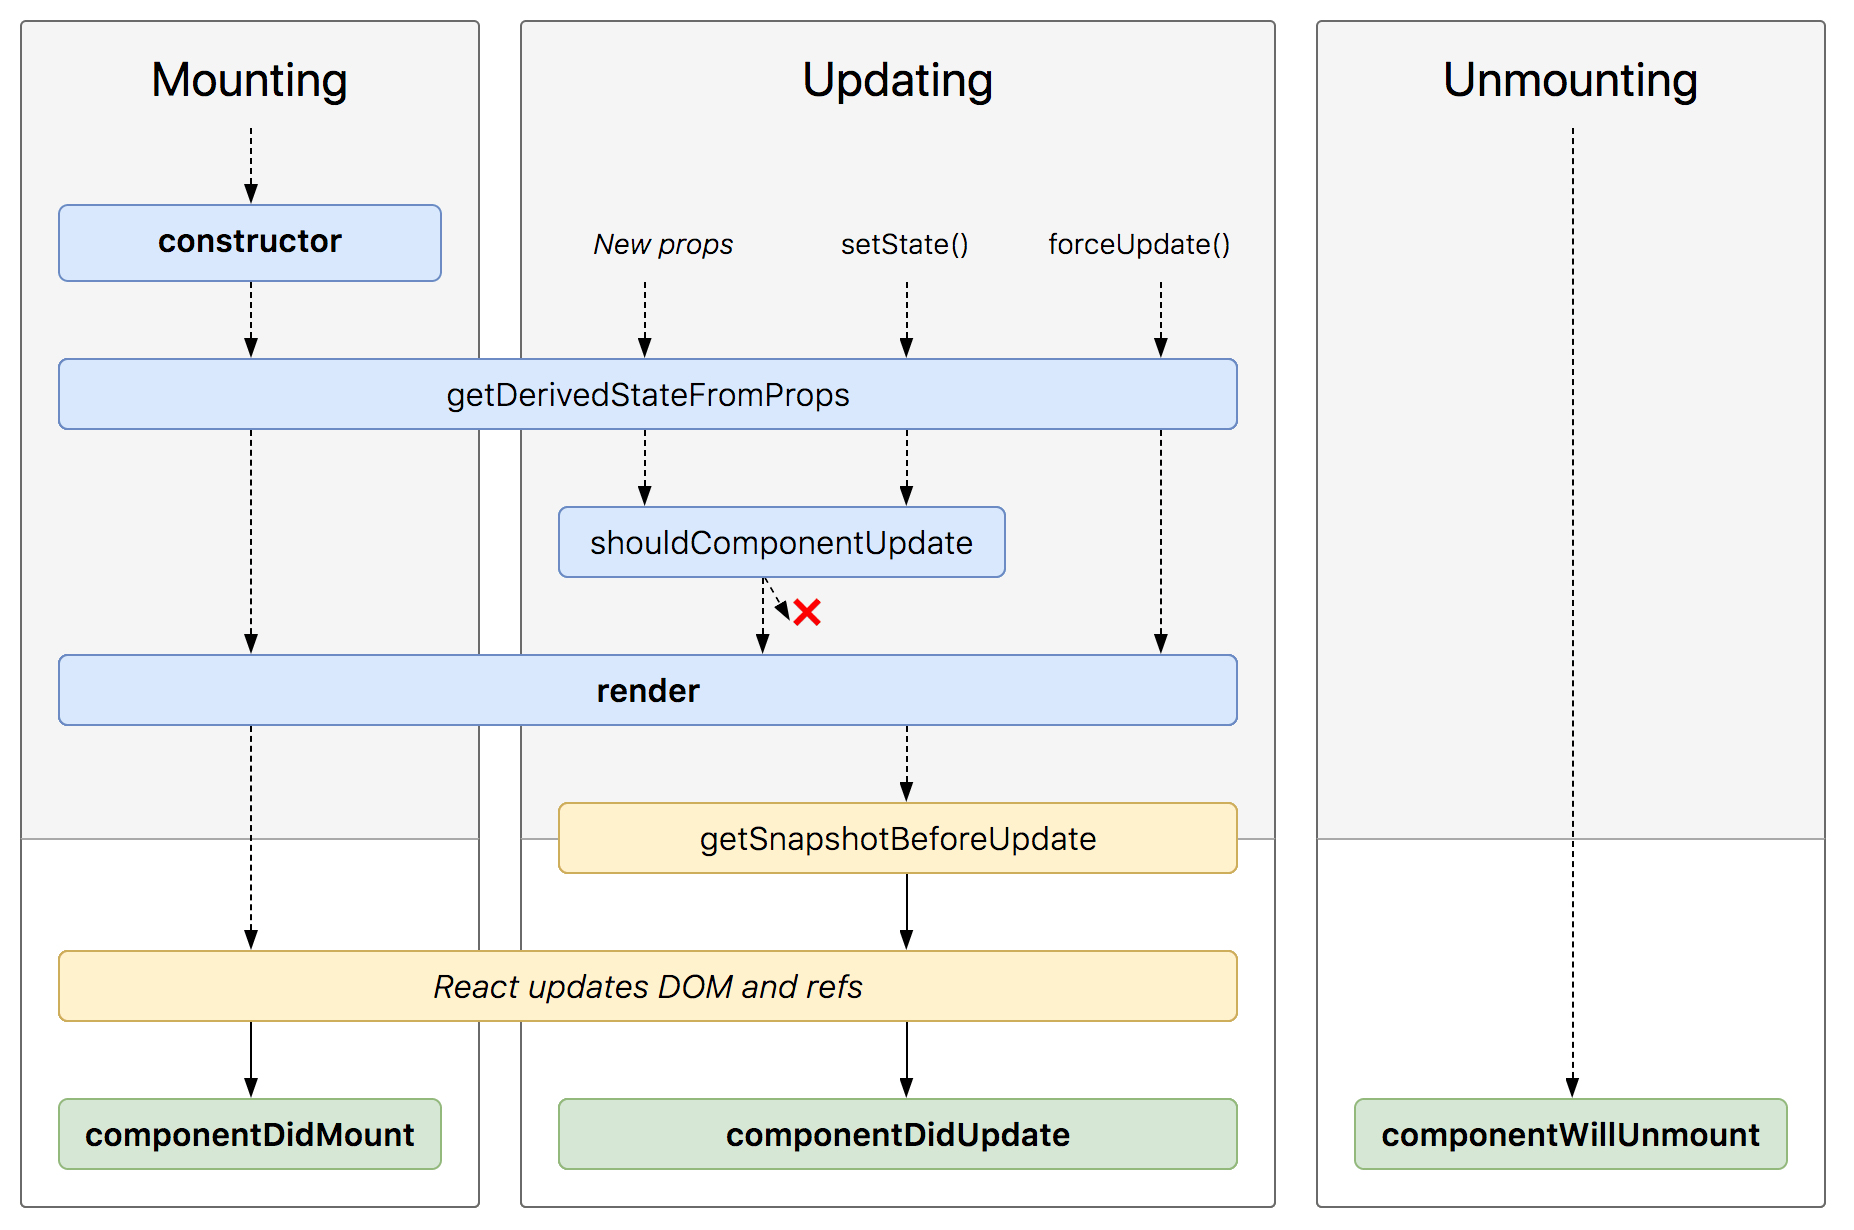
\includegraphics[scale=0.22]{main/images/lifecycleComponent.jpg}
\end{center}
\caption{Ciclo di vita di un componente.}
\label{fig:lifecycleComponent}
\end{figure}

Il costruttore è il primo metodo che viene chiamato. Per una corretta inizializzazione, all'interno del costruttore di un componente, dovremo innanzitutto invocare il costruttore della classe base \textit{super(props)} (come abbiamo visto definiamo un componente estendendo React.Component) passando le \textit{props} ricevute dal componente. 
Il secondo metodo ad essere invocato, immediatamente prima della funzione \textit{render()}, è \textit{componentWillMount()}. React consiglia di usare il costruttore al posto di questo metodo per ogni inizializzazione, poiché invocando la funzione \textit{setState()} all'interno di questo metodo gli altri \textit{licecycle hooks} non vengono richiamati.
La funzione \textit{render()} è l'unico metodo obbligatorio quando si vuole definire un componente. Non deve modificare direttamente l'oggetto \textit{props} o \textit{state}. All'interno della funzione render() non si deve manipolare il DOM o effettuare chiamate a funzioni per acquisire dati da un server. \textit{ComponentDidMount()} viene invocata dopo la funzione render(). Questo è il metodo da usare per manipolare il DOM o per recuperare eventuali dati da un server. Le valutazioni fatte in merito all'oggetto State nel metodo \textit{componentWillMount()} valgono anche per \textit{ComponentDidMount()}.

Quando viene aggiornato l'oggetto \textit{state} o in caso di ricezione di nuove \textit{props}, vengono invocati una serie di metodi in sequenza.
Il primo è \textit{shouldComponentUpdate()} che riceve come argomenti gli oggetti \textit{nextProps} e \textit{nextState} i quali rappresentano il prossimo valore dell'oggetto \textit{props} e dell'oggetto State. Il metodo \textit{shouldComponentUpdate()} restituisce un valore booleano. Se restituisce \textit{false}, i metodi successivi non verranno invocati. Di default questo metodo restituisce \textit{true}, consentendo l'aggiornamento del componente ad ogni modifica degli oggetti \textit{state} e \textit{props}. Per questo motivo, può essere usato per determinare se il componente deve essere aggiornato con i prossimi valori di \textit{props} e \textit{state}. All'interno di questo metodo è infatti possibile comparare i valori attuali degli oggetti \textit{state} e \textit{props} con quelli di \textit{nextState} e \textit{nextProps}, permettendo così di decidere se effettuare l'aggiornamento del componente, restituendo \textit{true} o \textit{false}.
Dopo il metodo render(), viene invocato \textit{componentDidUpdate()} che può essere usato per scaricare dati aggiornati da un server (nel caso per esempio ci sia stato un aggiornamento dell'oggetto \textit{props} o \textit{state}) o per operare sul DOM.

Nel fase di distruzione di un componente, invece, viene invocato come unico metodo \textit{componentWillUnmount()} che potremo usare per operazioni come invalidare eventuali timer avviati nella funzione \textit{componentDidMount()} e altre operazioni di manutenzione che prevengano memory leak.

\lstinputlisting[style=JavaScriptStyle]{main/code/lifecycleExample.js}

Il componente Clock nell'esempio imita il funzionamento di un orologio, mostrando a schermo la data
e l’ora corrente e aggiornandole ogni secondo. All’inizio del ciclo di vita del componente,
cioè quando questo viene montato per la prima volta nel DOM, viene richiamata la funzione \textit{componentDidMount()}, e il componente inizializza il proprio state, impostando
la data e l’ora.
Durante l’esecuzione di \textit{componentDidMount()} viene impostato un timer, che scatterà
ogni secondo fino a quando non viene fermato esplicitamente. Questo timer, ogni volta
che scatterà, chiamerà la funzione \textit{tick()} del componente. Questa funzione esegue a
sua volta un \textit{setState()}, e imposta anch’essa lo stato del componete con l’ora corrente.
Infine quando il componente viene rimosso dal DOM il timer viene fermato, in modo che
\textit{tick()} non venga più richiamato quando il componente verrà rimosso dal DOM e distrutto.

\subsection{Hooks}
\label{sec:hooks}

Gli Hooks sono stati aggiunti in React 16.8 e permettono di utilizzare \textit{state} ed altre funzioni di React senza dover scrivere un componente sottoforma di classe. Gli Hooks sono funzioni che ti permettono di “ancorarti” all’interno delle funzioni di React state e lifecycle da componenti funzione. 

Uno degli hooks fondamentali è \textit{useState}, un Hook che ti permette di aggiungere lo state React nei componenti funzione. L’unico argomento per l’Hook useState() è lo stato iniziale. A differenza delle classi, lo state non deve essere un oggetto. Possiamo tenere un numero o una stringa se è quello di cui abbiamo bisogno. La \textit{useState} ritorna una coppia di valori: lo stato corrente ed una funzione che lo aggiorna. Questi due valori vengono assegnati ad un array grazie alla sintassi JavaScrypt chiamata destrutturazione di array.

\lstinputlisting[style=JavaScriptStyle]{main/code/hookExample.js}

Grazie a \textit{useState()} ora è possibile definire componenti funzione con il proprio stato. L'unico grosso vantaggio che posseggono i componenti di classe sono i metodi lifecycle. Per ovviare a questa mancanza è stato introdotto l'hook \textit{useEffect()} che offre la possibilità di comportamenti simili alle funzioni \textit{componentDidMount()}, \textit{componentDidUpdate()} e \textit{componentWillUnmount()}.
L'hook \textit{useEffect()} accetta due argomenti: il primo argomento è una funzione callback che viene eseguita  dopo il render del componente; mentre il secondo argomento è un array di valori, solitamente corrispondenti alle \textit{props}. Se l'array non viene espresso la callback viene invocata dopo ogni render; quando l'array è presente ma non contiene alcun elemento la callback viene richiamata solo alla creazione del componente (\textit{componentDidMount()}). Se invece, l'array contiene dei valori, la funzione viene eseguita solamente alla variazione di almeno una delle variabili specificate in esso (\textit{componentDidUpdate()}). Se, come valore di ritorno della funzione di callback, viene definita una ulteriore funzione, questa viene eseguita appena prima della distruzione del componente imitando il ruolo del metodo \textit{componentWillUnmount()}.

Il codice riportato sotto riprende l'esempio mostrato nel paragrafo del ciclo di vita del componente, rivisto con l'utilizzo degli hook.

\lstinputlisting[style=JavaScriptStyle]{main/code/hookEffectExample.js}

\subsection{Routing}
\label{sec:routing}
Grazie all'utilizzo della libreria React è possibile sviluppare le cosiddette "single-page application", cioè applicazioni che si basano su una singola pagina HTML. Nel caso di React questo è possibile grazie al render di componenti diversi all'interno del medesimo elemento HTML, dando l'impressione all'utente di spostarsi in pagine differenti. 

Questo lavoro è agevolato dalla libreria React-router\footnote{React-router: \url{https://reacttraining.com/react-router/}} offrendo una collezione di API completa e semplice da usare. 

L'integrazione di questa libreria porta con sé vantaggi e svantaggi. La possibilità di creare una "single-page application" permette di evitare richieste HTTP al web server per ogni reindirizzamento di pagina, rendendo più fluida ed intuitiva la navigazione. Al contempo, la web application dev'essere caricata nella sua interezza ad ogni visita, anche se alcune pagine non vengono utilizzate. Questo può essere un grosso difetto per applicazioni web di grandi dimensioni poiché i tempi di caricamento iniziale si dilaterebbero notevolmente.

\subsection{Il pattern Flux}
\label{sec:flux}

Flux è l'architettura dell'applicazione che React utilizza per creare applicazioni Web sul lato client. Completa i componenti della UI di React utilizzando un flusso di dati unidirezionale.

Le applicazioni Flux hanno tre parti principali: il \textit{dispatcher}, gli \textit{store} e le \textit{view} (componenti React). Questi non devono essere confusi con le entità che compongono MVC (Model View Controller), pattern maggiormente diffuso per strutturazione di software che utilizza elementi grafici. I controller esistono in un'applicazione Flux, ma sono fortemente legati alle \textit{view}, cioè ai componenti React.

Flux evita gli standard del pattern MVC a favore di un flusso di dati unidirezionale. Questa scelta è dovuta al fatto che la maggior parte dei framework JavaScript, tra cui React, fornisce il supporto per l'associazione dei dati che consente alla vista di dialogare direttamente con il modello. L'adozione di MVC, quindi, renderebbe lo sviluppo e il debug di applicazioni di dimensioni importanti molto difficoltosa.
Quando un utente interagisce con una vista React, la vista propaga un'azione attraverso un \textit{dispatcher} centrale, ai vari \textit{store} che contengono i dati dell'applicazione e la logica di business. A sua volta aggiorna tutte le \textit{view} interessate. Funziona particolarmente bene con lo stile di programmazione dichiarativo di React, che consente all'archivio di inviare aggiornamenti senza specificare come passare da una vista all'altra.

\begin{figure}
\begin{center}
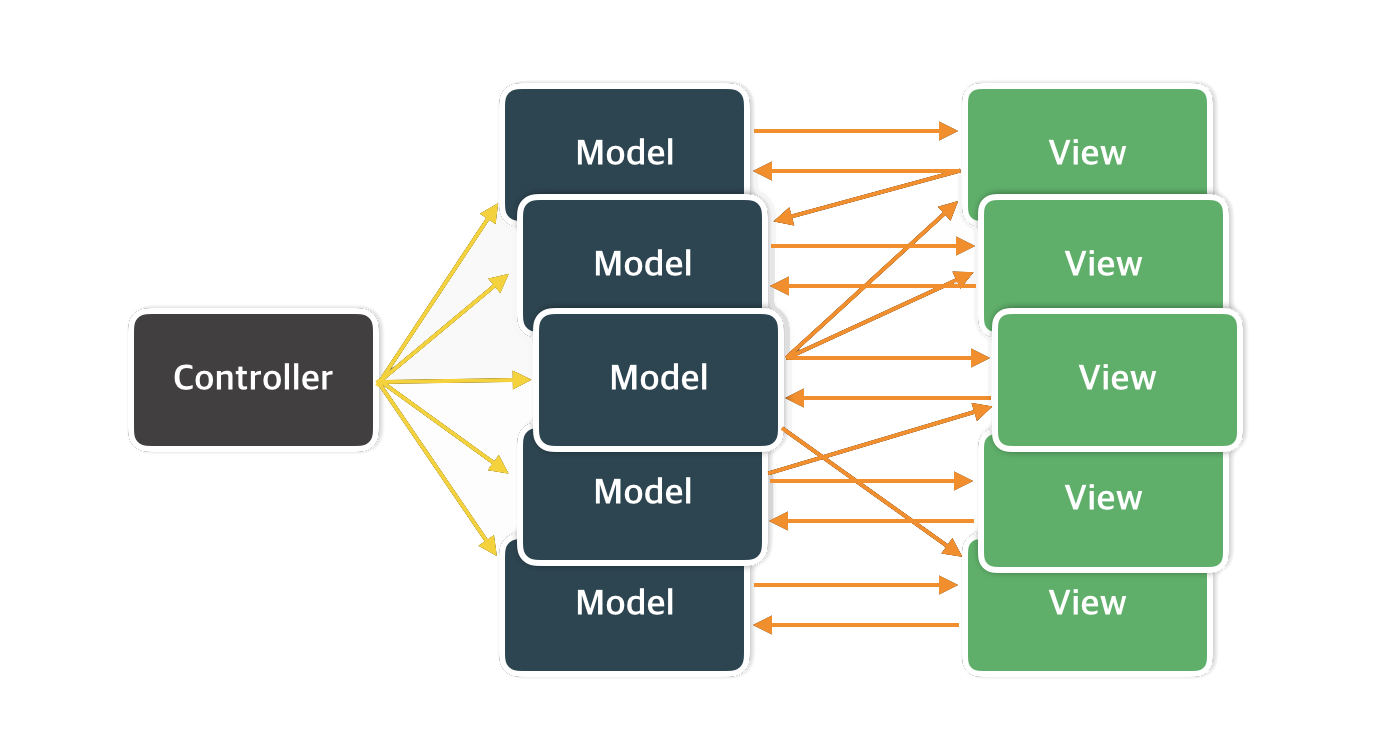
\includegraphics[scale=0.3]{main/images/mvc.png}
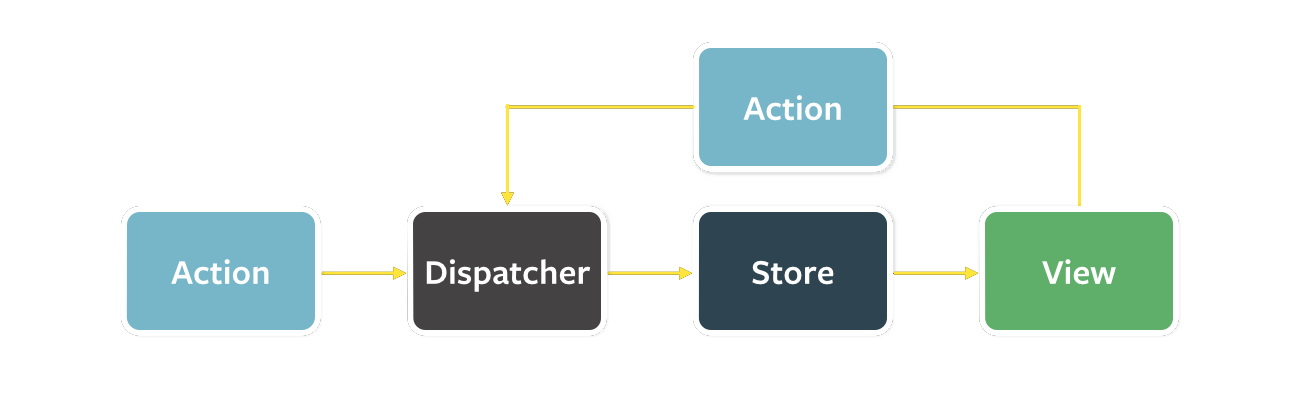
\includegraphics[scale=0.3]{main/images/flux.png}
\end{center}
\caption{Struttura del pattern MVC (in alto) e Struttura del pattern Flux (in basso).}
\label{fig:pattern}
\end{figure}

Un flusso di dati unidirezionale è fondamentale per il modello Flux. Il \textit{dispatcher}, i \textit{negozi} e le \textit{view} sono nodi indipendenti con input e output distinti. Le azioni sono oggetti JavaScript semplici contenenti i nuovi dati e una proprietà \textit{type} che identifica la tipologia dell'azione.

Le \textit{view} possono causare una nuova azione da propagare attraverso il sistema in risposta alle interazioni dell'utente. Tutti i dati passano attraverso il \textit{dispatcher} come un hub centrale.  Il \textit{dispatcher} quindi richiama le funzioni di callback che gli \textit{store} hanno registrato con esso. All'interno delle callback registrate, gli \textit{store} rispondono a qualsiasi azione rilevante per lo stato che contengono. Gli \textit{store} emettono quindi un evento di modifica per avvisare i componenti che si è verificata una modifica al livello dati. Le \textit{view} invocano il proprio metodo \textit{setState()}, causando un nuovo rendering di se stessi e di tutti i loro discendenti nella struttura dei componenti.

\subsection{Integrazione in OVL Dashboard}
\label{sec:integragrazione in OVL Dashboard}

Di seguito è riportata l'implementazione del componente \textit{ticket} di OVL Dashboard. È possibile notare l'utilizzo di svariati hook \textit{useState()} per tenere traccia di tutti gli aspetti di un ticket ed effettuare il re-render ad ogni loro cambiamento. Particolare, inoltre, è l'utilizzo di due differenti hook \textit{useEffect()} che eseguono le proprie callback alla variazione di \textit{state} e \textit{props} differenti: il primo aggiorna l'aspetto del ticket a seconda delle informazioni che contiene, mentre il secondo inizializza alcune variabili utilizzate in porzioni successive di codice.

\lstinputlisting[style=JavaScriptStyle]{main/code/ticketExample.js}

\section{Redux}
\label{sec:redux}

Durante lo sviluppo di OVL Dashboard ho deciso di utilizzare la libreria
Redux per semplificare lo sviluppo riguardante la gestione dello stato dell'applicazione. Di seguito, verranno illustrate le motivazioni che hanno portato a questa decisione
e verrà descritto il funzionamento di questa libreria. 
Redux è un'evoluzione di Flux, ne condivide alcuni dei principi, tra cui il concetto di flusso unidirezionale delle informazioni, ma si differenzia per alcuni aspetti importanti.

Senza l'utilizzo di Redux, ogni componente dovrebbe mantenere e gestire il proprio stato e la comunicazione con gli altri componenti avverrebbe esclusivamente tramite \textit{props}. Con l'introduzione di questa libreria nasce il concetto di avere un unico stato, rappresentato da un oggetto JSON e conservato in uno store. Questo stato può mutare solo in seguito ad azioni, ma non può essere modificato direttamente. La modifica avviene tramite l’invocazione di una funzione denominata reducer.

\begin{figure}
\begin{center}
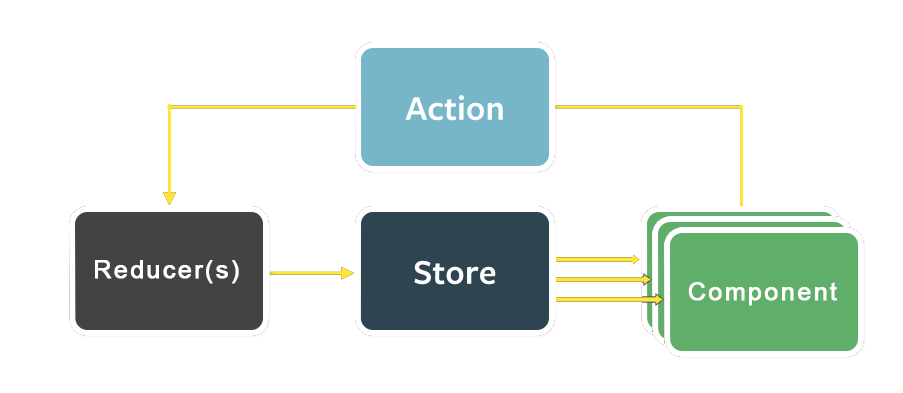
\includegraphics[scale=0.45]{main/images/redux.png}
\end{center}
\caption{Render in Redux.}
\label{fig:reduxFlow}
\end{figure}

Con Redux vengono introdotti diversi termini e concetti che è importante analizzare uno per uno.

Lo \textit{state} è quello conosciuto già in React, cioè lo stato che viene renderizzato nell'interfaccia. È buona pratica, e Redux serve proprio a questo, mantenere lo stato generale dell'applicazione nel modo più centralizzato possibile.

Le \textit{action} sono semplici oggetti JavaScript utilizzati per inviare informazioni allo \textit{store}. Si tratta dell'unico mezzo attraverso il quale si può richiedere l'aggiornamento delle informazioni presenti nello \textit{store} che è l'oggetto che mantiene lo stato dell'intera applicazione. L'unico requisito delle \textit{action} è che devono essere un oggetto contenente una proprietà \textit{type} che è la sola proprietà necessaria affinché un oggetto possa definirsi un'\textit{action}. Oltre alla proprietà \textit{type}, possiamo aggiungere altre proprietà, a seconda delle necessità e delle informazioni che vogliamo passare ai \textit{reducer}.

\lstinputlisting[style=JavaScriptStyle]{main/code/actionExample.js}

I \textit{reducer} sono le uniche funzioni autorizzate ad aggiornare le informazioni contenute nello \textit{store} il quale è l'oggetto predisposto a mantenere lo stato dell'intera applicazione.
È importante sottolineare che le funzioni \textit{reducer} non modificano l'oggetto State, ma ricevono in ingresso l'oggetto State corrente e restituiscono un nuovo oggetto \textit{state}. 
Al fine di gestire correttamente lo state centralizzato occorre creare una funzione \textit{reducer} per ogni pezzo dell'oggetto State e poi combinare tali funzioni in un unico \textit{reducer}.

\lstinputlisting[style=JavaScriptStyle]{main/code/reducerExample.js}

Lo \textit{store} è l'oggetto che mantiene lo \textit{state} dell'applicazione e fornisce alcuni metodi come \textit{getState()}, che restituisce l'oggetto \textit{state} dell'applicazione e \textit{dispatch(action)} che serve per lanciare un'\textit{action}. Lo \textit{store} ha inoltre un metodo \textit{subscribe(listener)} che serve per registrare una funzione che verrà invocata ogni volta che un'\textit{action} verrà lanciata da \textit{dispatch(action)}.

L'utilizzo della libreria Redux quindi permette di avere un oggetto unico, centralizzato a cui possono accedere più componenti contemporaneamente. Lo \textit{store} centrale e condiviso diminuisce notevolmente la complessità dei singoli componenti e riduce la duplicazione dei dati nel caso di componenti che necessitano delle medesime informazioni.

\subsection{Integrazione in OVL Dashboard}
\label{sec:integragrazione in OVL Dashboard}

Nei progetti importanti come quello trattato in questo lavoro, l'utilizzo del sistema della libreria Redux è fortemente legato al ruolo dei dati trattati all'interno del progetto. L'adozione di Redux è ottimale se l'informazione rappresentata è utile a più componenti e se serve mantenere le variabili anche dopo la distruzione dei componenti. Inoltre, nello \textit{store} Redux è possibile mantenere una sorta di cronologia delle azioni invocate. Al contrario, lo \textit{state} locale viene mantenuto per tenere traccia dei dati nel corso della vita di un certo componente, quindi da un certo punto di vista "temporanei".

La struttura dello stato in OVL Dashboard riflette quanto consigliato dalle
linee guida di Redux: un oggetto con diverse proprietà, ognuna delle quali rappresenta
una porzione dello stato indipendente dalle altre dal punto di vista logico. Queste sono:
\begin{itemize}
    \item \textit{oidc} contiene le informazioni riguardo allo stato di autenticazione dell'utente ed i dati di profilo associati ad esso (forniti dal server di autorizzazione) 
    \item \textit{invitations} contiene le informazioni riguardanti i nuovi inviti effettuati
    \item \textit{groups} contiene i gruppi delle connessioni a cui l'utente corrente ha accesso
    \item \textit{groupsConnections} contiene i gruppi e le relative connessioni a cui l'utente corrente ha accesso
    \item \textit{tickets} contiene lo stato dei ticket
\end{itemize}

Gli oggetti \textit{groups}, \textit{groupsConnections} e \textit{ticket} permettono di mantenere le rispettive informazioni fino alla chiusura della pagina in modo da effettuare il caricamento dei dati dal database solamente alla prima creazione dei componenti.

Di seguito un esempio dello stato dell'oggetto \textit{tickets}:

\lstinputlisting[style=JsonStyle]{main/code/ticketStore.json}

L'oggetto Json riportato mostra due oggetti ticket contenenti i campi riferiti allo stato e alla tipologia della richiesta e i campi necessari all'aggiunta della nuova connessione in caso il ticket venga accettato.

\section{WebRTC}
\label{sec:WebRTC}

Per la progettazione della pagina di assistenza, in particolare per l'implementazione della fase di comunicazione, si è scelto di adottare la libreria WebRTC (Real-Time Communications).
Le specifiche WebRTC nascono con l’intento di offrire agli sviluppatori web uno strumento per gestire lo scambio di flussi di dati (in primo luogo quelli multimediali come audio e video) tra due dispositivi in collegamento diretto peer-to-peer.

WebRTC offre tre API principali, utili per l'inizializzazione della comunicazione:
\begin{itemize}
    \item \textit{getUserMedia} consente di ottenere un flusso audio/video proveniente dalla telecamera e dal microfono installato sul device dell’utente 
    \item \textit{RTCPeerConnection} gestisce la connessione e la comunicazione di flussi di dati tra due dispositivi in connessione peer-to-peer
    \item \textit{RTCDataChannel} consente l’interscambio di flussi di dati arbitrari tra due dispositivi in connessione peer-to-peer
\end{itemize}

\begin{figure}
\begin{center}
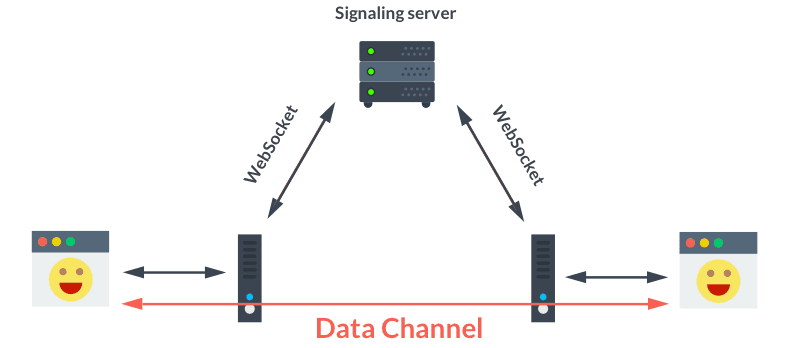
\includegraphics[scale=0.6]{main/images/WebRTC.png}
\end{center}
\caption{struttura di WebRTC.}
\label{fig:reduxFlow}
\end{figure}

Per instaurare la connessione, il sistema di WebRTC necessita in primo luogo di un signaling server. Questo server è un websocket server che permette l'interazione tra due client al fine di organizzare e impostare la comunicazione. 
Prima che due parti possano avviare una videochiamata o una chiamata, una parte deve contattare l'altra e la parte contattata deve rispondere. Questo procedimento avviene mediante un protocollo basato su offerta-risposta gestito totalmente dal signaling server.
Quando il chiamante riceve il messaggio di risposta dal ricevente, viene instaurata la connessione peer-to-peer per lo scambio di flussi di dati.

I client inizialmente si registrano presso il signaling server inviandogli un identificativo. 
La configurazione di un endpoint su una connessione WebRTC è chiamata descrizione della sessione. La descrizione include informazioni sul tipo di supporto inviato, il suo formato, il protocollo di trasferimento utilizzato, l'indirizzo IP e la porta dell'endpoint e altre informazioni necessarie per descrivere un endpoint di trasferimento multimediale. Queste informazioni vengono scambiate e archiviate utilizzando Session Description Protocol (SDP). Quando un utente avvia una chiamata WebRTC a un altro utente, viene creata una descrizione speciale chiamata offerta. Questa descrizione include tutte le informazioni sulla configurazione proposta del chiamante. Il destinatario, quindi, manda una risposta che contiene una descrizione delle informazioni sulla propria configurazione. In questo modo, entrambi i dispositivi condividono tra loro le informazioni necessarie per scambiare dati multimediali. Questo scambio viene gestito utilizzando Interactive Connectivity Establishment (ICE), un protocollo che consente a due dispositivi di utilizzare un intermediario per scambiare offerte e risposte. Ogni peer, quindi, tiene a portata di mano due descrizioni: la descrizione locale, che descrive se stessa, e la descrizione remota, che descrive l'altra estremità della chiamata.
Oltre allo scambio di informazioni sui media, i peer devono scambiarsi informazioni sulla connessione di rete. Questo è noto come candidato ICE e descrive in dettaglio i metodi disponibili che il peer è in grado di comunicare.
\chapter{Tecnologie di sviluppo del back-end}
\label{chap:tecnologie di sviluppo del back-end}

L’architettura scelta per OVL Dashboard segue il modello client-server, in cui il client rappresenta l’interfaccia, mentre il server svolge il compito di implementazione delle logiche applicative e di conservazione dei dati. La comunicazione tra le due componenti avviene tramite Internet, in modo tale da permettere a qualunque utente della piattaforma di raggiungerla facilmente dal dispositivo e dal luogo che preferisce.

Il back-end di OVL Dashboard è composto, come visto in precedenza, da diversi elementi: il server di storage, il server di autenticazione, un database MySQL per la memorizzazione delle connessioni e un secondo database noSQL per la gestione degli utenti. Tutti questi apparati sono mantenuti all'interno del cloud computing di AWS (Amazon Web Services)\footnote{AWS: \url{https://aws.amazon.com}}.

Il server di storage offre gli endpoint necessari a soddisfare i vari casi d'uso provenienti dal front-end, cioè dalla dashboard. Esso permette l'effettiva gestione delle connessioni della rete virtuale mediante la comunicazione con il database MySQL (condiviso e gestito con Guacamole).

Il server di autorizzazione, invece, rende possibile l'accesso a tutti i servizi di OpenVirtualLab con l'utilizzo di un singolo account. Questo server è implementato partendo da un fork del progetto OpenID Connect, che consente ai client di tutti i tipi, inclusi client Web, mobili e JavaScript, di richiedere e ricevere informazioni su sessioni autenticate e utenti finali. L'adozione di un server di autenticazione permette di mantenere separati la logica di gestione degli account e le funzionalità legate ad essi dai servizi OVL dell'azienda Themis s.r.l. Per la memorizzazione delle informazioni relative agli account è stato utilizzato MongoDB, un database documentale che offre alte prestazioni.

\section{AWS}
\label{sec:AWS}

Con il termine “cloud computing” si indicano una serie di tecnologie che permettono di elaborare, archiviare e memorizzare dati grazie all'utilizzo di risorse hardware e software distribuite nella rete.
L’innovazione apportata dalle configurazioni cloud riguarda la distribuzione in rete dei servizi, la semplice scalabilità dell'infrastruttura, le maggiori affidabilità e continuità del servizio e l’erogazione in tempi molto rapidi di nuove risorse di calcolo e memorizzazione.
Con servizi cloud si intendono server pilotati da un software che ne mette a disposizione le capacità di calcolo (CPU) e di memorizzazione (dischi); i servizi forniti vengono dislocati automaticamente tra tutti i server disponibili e in caso di necessità nuovi server possono essere facilmente aggiunti per aumentare la capacità complessiva del sistema. In particolare, AWS è una piattaforma di servizi cloud sicura in grado di offrire potenza di elaborazione, storage di database, distribuzione dei contenuti e altre funzionalità a supporto del dimensionamento e della crescita delle attività aziendali.
Il servizio per eccellenza di AWS è rappresentato da EC2, Elastic Computing Cloud. Esso è un servizio di AWS che fornisce un’infrastruttura web per disporre di macchine virtuali completamente on demand. Tramite EC2 è possibile configurare, avviare, spegnere e clonare istanze di macchine virtuali costruite totalmente secondo le proprie necessità. Per quanto riguarda i servizi di database abbiamo usato RDS (Amazon Relational Database Service), che è un servizio che semplifica configurazione, utilizzo e ridimensionamento di database relazionali nel cloud. Offre capacità ridimensionabili ad un costo vantaggioso e gestisce al contempo lunghe attività amministrative del database, in modo da consentire all'utente di concentrarsi sulle proprie applicazioni e sul proprio business. Amazon RDS permette di scegliere tra sei motori di database comuni: Amazon Aurora, PostgreSQL, MySQL, MariaDB, Oracle e Microsoft SQL Server. I due servizi appena descritti sono stati quelli di maggior interesse per lo sviluppo della dashboard.

\section{Node.js e Express}
\label{sec:Node.js e express}

Per lo sviluppo dei entrambi i server è stato adottato Node.js, un’applicazione, per la precisione un framework, nata nel 2009, che viene usata per scrivere applicazioni in Javascript lato server.
Il codice su Node.js, infatti, viene fatto girare da V8. Sto parlando del motore JavaScript open source di Google, scritto in C++ e utilizzato in Google Chrome. Si tratta di una soluzione lato server basata su un modello di I/O asincrono che opera sugli eventi. Node richiede al sistema operativo di ricevere notifiche al verificarsi di determinati eventi, e rimane quindi in attesa fino alla notifica stessa: solo in tale momento torna attivo per eseguire le istruzioni previste in una funzione di callback, così chiamata perché da eseguire una volta ricevuta la notifica che il risultato dell'elaborazione del sistema operativo è disponibile.
Nonostante un singolo processo Node.js venga sempre eseguito su un singolo thread, sui sistemi multicore è possibile creare un cluster. Per fare ciò l’applicazione Node.js crea un insieme di processi figli detti worker e suddivide le connessioni in entrata in modo equo tra di essi.
In gran parte dei server web, le operazioni di I/O sono bloccanti: il thread del server viene infatti bloccato dal sistema operativo per il tempo necessario alla conclusione dell’operazione. Questo problema è stato risolto rendendo i web server multi-threaded, e creando un thread per ogni connessione. La creazione e la gestione di thread però non è sempre efficiente, soprattutto in caso si grandi quantità di connessioni. Node.js invece utilizza un modello orientato agli eventi, e questo gli consente di compiere le operazioni di I/O in modo non bloccante nonostante venga eseguito su un singolo thread. Ogni operazioni di I/O è infatti asincrona: l’operazione viene fatta partire, ed è necessario registrare una funzione di callback che verrà richiamata da Node.js appena l’operazione sarà terminata. Questa caratteristica lo rende particolarmente efficiente per le applicazioni web, in cui le operazioni di rete sono frequenti e di vitale importanza.

Insieme a Node.js è stato utilizzato Express, un web framework minimale e flessibile, che offre strumenti di base per creare più velocemente applicazioni in Node.
Express mette a disposizione dei Routers, sulle quali posso definire le mie rotte, i miei endpoint dei servizi. La loro struttura è molto semplice. Occorre specificare per ogni endpoint il metodo di richiesta http, il path della route e la funzione handler da eseguire al match della route.  

La scelta di Node.js ha sicuramente accelerato lo sviluppo. L’utilizzo di un linguaggio di programmazione comune sia dal lato client che dal lato server ha consentito alla parte di team che si occupa del front-end di revisionare, eseguire il debug e in alcuni casi contribuire alla parte back-end dell'applicazione senza la necessità di dover apprendere un altro linguaggio di programmazione. Lavorare con Express poi semplifica notevolmente la realizzazione di applicazioni web, che grazie a Router permette di strutturare bene le risorse.

\section{Guacamole}
\label{sec:guacamole}

Guacamole è un'applicazione Web HTML5 che fornisce l'accesso agli ambienti desktop mediante protocolli desktop remoti (come VNC o RDP). Guacamole consente l'accesso a uno o più desktop da qualsiasi luogo in remoto, senza dover installare un client, in particolare quando l'installazione di un client non è possibile. Questa piattaforma, inoltre, mette a disposizione le funzionalità per la gestione di gruppi di utenti e di conseguenza permette di definire permessi differenti tra utenti e dispositivi accessibili da remoto. 

\begin{figure}
\begin{center}
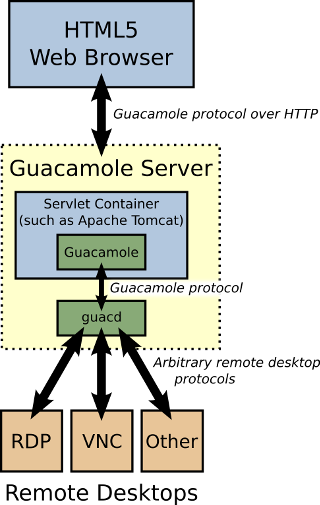
\includegraphics[scale=2]{main/images/guac-arch.png}
\end{center}
\caption{Architettura Guacamole.}
\label{fig:lifecycleComponent}
\end{figure}

La figura 4.1 mostra l'architettura di Guacamole. Si può notare in alto il client web per il monitoraggio delle connessioni e del loro stato. 

Il componente Guacd, all'interno del server, è il cuore di Guacamole che carica in modo dinamico il supporto per i protocolli desktop remoti (chiamati "plug-in client") e li collega ai desktop remoti in base alle istruzioni ricevute dall'applicazione web.
Guacd è un processo daemon che viene installato insieme a Guacamole e viene eseguito in background, ascoltando le connessioni TCP dall'applicazione Web. Guacd inoltre non comprende alcun protocollo specifico per desktop remoto, ma implementa abbastanza il protocollo Guacamole per determinare quale supporto di protocollo deve essere caricato e quali argomenti devono essere passati ad esso. Una volta caricato un plug-in client, viene eseguito indipendentemente da Guacd e ha il pieno controllo della comunicazione tra se stesso e l'applicazione Web fino al termine del plug-in client.

Guacamole è l'applicazione a cui si appoggia OVL Dashboard per instaurare le connessioni remote ai dispositivi. Esso mantiene le informazioni riguardanti utenti, permessi e dispositivi remoti in un database MySQL. Le funzionalità implementate in OVL Dashboard rendono possibile la completa gestione di queste informazioni, oltre a donare al sistema Guacamole un'interfaccia web più moderna e intuitiva.
\chapter{Conclusioni}
\label{chap:conclusioni}

Nella prima versione di OVL Dashboard io ed il mio collega siamo riusciti ad ottenere un versione completa e funzionante dal punto di vista della gestione delle connessioni e della comunicazione real-time sulla piattaforma.
Innanzitutto, si è deciso di adottare React come libreria principale per la realizzazione dell'interfaccia grafica. Questa soluzione ha permesso di suddividere l’applicazione in componenti riutilizzabili ed estendibili, migliorando l’efficienza dell'attività di sviluppo e consentendo una facile manutenzione del codice. Infine, per la gestione della logica applicativa, l’utilizzo di Redux ha consentito di gestire in modo facile la gestione dello stato dell'applicazione, contribuendo a rendere l’applicazione più modulare e a prevenire l’introduzione di alcuni tipi di bug e di codice ridondante. È stato fondamentale comprendere in modo completo tutti i punti di forza di React al fine di sfruttarlo a pieno e rendere la web application intuitiva e performante. 

\section{Sviluppi futuri}
\label{sec:sviluppi futuri}
Gli sviluppi futuri della piattaforma sono molteplici. Dal punto di vista delle funzionalità si punta a trasformare la dashboard in modo da renderla un elemento fondamentale nelle attività mediche quotidiane. In particolare occorre implementare la comunicazione real-time, non solamente come chiamato vocale o testuale, ma anche come streaming video. Questo permetterebbe un'eventuale consulenza tra medici con l'ausilio aggiuntivo del video in tempo reale per diagnosi di soggetti sotto osservazione. Ampliando ancora di più la visione di utilizzo di questo strumento è possibile equipaggiare i mezzi di soccorso medico con dispositivi dotati di connettività mobile per collegarsi alla dashboard ed ottenere un'opinione di uno specialista su un particolare caso clinico.
Inoltre, verrà aggiunta la possibilità da parte degli utenti amministratori di creare e gestire istanze di macchine virtuali grazie alle SDK del servizio EC2 offerte da AWS.
Dal punto di vista della sicurezza e del monitoraggio delle attività svolte all'interno della dashboard, viene utilizzata una blockchain privata basata su una rete Ethereum\footnote{Ethereum: \url{https://www.ethereum.org/}}. All'interno della blockchain, attualmente già implementata, verranno scritte e mantenute nel tempo tutte le operazioni eseguite dagli utenti all'interno di OVL Dashboard, garantendo la sicurezza delle informazioni. L'adozione di questa  tecnologia permette inoltre di avere uno storico, presentato sotto forma di log all'interno della piattaforma visibile solamente dall'account dell'azienda.


%%%%%%%%%%%%%%%%%%%%%%%%%%%%%%%%%%%%%%%%%%%%%%%%%%%%%%%%%%%%%%%

% BIBLIOGRAFIA
\phantomsection
\addcontentsline{toc}{chapter}{\refname}
\nocite{*}
\printbibliography

\end{document}